\documentclass{article}

% Configuração de idioma
\usepackage[brazil]{babel}

% Ajuste de margens
\usepackage[letterpaper,top=2cm,bottom=4cm,left=2cm,right=2cm]{geometry}

% Pacotes úteis
\usepackage{amsmath}
\usepackage{graphicx}
\usepackage[colorlinks=true, allcolors=blue]{hyperref}
\usepackage[nice]{nicefrac}
\usepackage{float}
\usepackage{booktabs}
\usepackage{enumerate}
\usepackage{fancyhdr}  % Customização de cabeçalhos e rodapés
\usepackage{xcolor}  % Definição de cores
\usepackage{multirow} % Para tabelas com múltiplas linhas
\usepackage{titling}  % Permite ajustar espaçamento do título

% Definição de cores institucionais
\definecolor{IFSCgreen}{RGB}{0,104,56}
\definecolor{IFSCgreenweak}{RGB}{97,154,132}

% Ajuste da altura do cabeçalho para evitar sobreposição
\setlength{\headheight}{2.5cm}

% Reduz o espaço entre o cabeçalho e o título
\setlength{\droptitle}{-1.5cm}

% Configuração do cabeçalho
\pagestyle{fancy}
\fancyhf{} % Limpa o cabeçalho e rodapé padrão
\fancyhead[L]{ % Cabeçalho alinhado à esquerda
    \begin{tabular}{p{10.5cm}r}
        \multirow{4}{*}{
\includegraphics[width=6cm]{IFSCLogo}} &  \\ 
        & \footnotesize \fontfamily{phv}\fontseries{mc}\selectfont\small \textcolor{IFSCgreenweak}{Ministério da Educação} \\ 
        & \footnotesize\fontfamily{phv}\fontseries{mc}\selectfont\small \textcolor{IFSCgreenweak}{Secretaria de Educação Profissional e Tecnológica} \\ 
        & \small\fontfamily{phv}\fontseries{mc}\selectfont\large \textcolor{IFSCgreen}{INSTITUTO FEDERAL DE SANTA CATARINA} \\
    \end{tabular}
}
\renewcommand{\headrulewidth}{0pt} % Remove a linha horizontal do cabeçalho

% Título e autor
\title{\textbf{Título do Trabalho}}
\author{Autor(a) \\ [0.5em] Trabalho submetido à UC de Sistemas de Controle (20xx/x)}
\date{}

\begin{document}

\maketitle
\thispagestyle{fancy}



\section{Introdução}


 

\begin{align}
    y &= x^{2} +\int_{1}^{2} \lambda \partial x \\
    x &= a_{0} + \sum_{n=1}^{\infty} a_{n} \cos\left(n\frac{\pi}{2} t\right) +b_{n} \sin(n\omega_0 t) \notag \\
    \frac{Y(s)}{U(s)} &= \frac{K\omega_0^2}{s^2 +2\zeta\omega_0 s +\omega_0^2} \\
    u(t) &= k_p e(t) +k_i\int e(t) dt +k_d \frac{de(t)}{dt} \label{eq:one}
\end{align}


\begin{align}
     y=\begin{cases}
 1, & \text{ se }\quad x= 0,\\
 2, & \text{ se }\quad x= 10,\\
 3, & \text{ se }\quad x= 20.
\end{cases}
\end{align}

\begin{align}
    \dot{x} &= \begin{bmatrix}
0 & 1 \\
-2 & -3 \\
\end{bmatrix} x + \begin{bmatrix}
0 \\
1
\end{bmatrix} u \\
y &= \begin{bmatrix}
0 & 1 \\
\end{bmatrix} x
\end{align}





Na introdução $\nicefrac{Y(s)}{U(s)} = \nicefrac{K\omega_0^2}{s^2}$ a equipe tem que informar o que foi proposto para o projeto de forma clara e dizer, também de forma clara, como as diferentes disciplinas estudadas até aqui se relacionam dentro do projeto escolhido para ser trabalhado. 

\begin{table}[H]
  \centering
  \caption{Characteristics of feeder JSL07}
    \begin{tabular}{cc}
    \toprule
    \textbf{Description} & \textbf{Quantity} \\
    \midrule
    Medium voltage segments & 148 \\
    Low voltage segments & 171 \\
    Distribution transformer units & 24 \\
    Medium voltage transformer units & 13 \\
    Low voltage transformer units & 604 \\
    \bottomrule
    \end{tabular}%
  \label{tab:jsl07}%
\end{table}%

\begin{figure}[H]
    \centering
    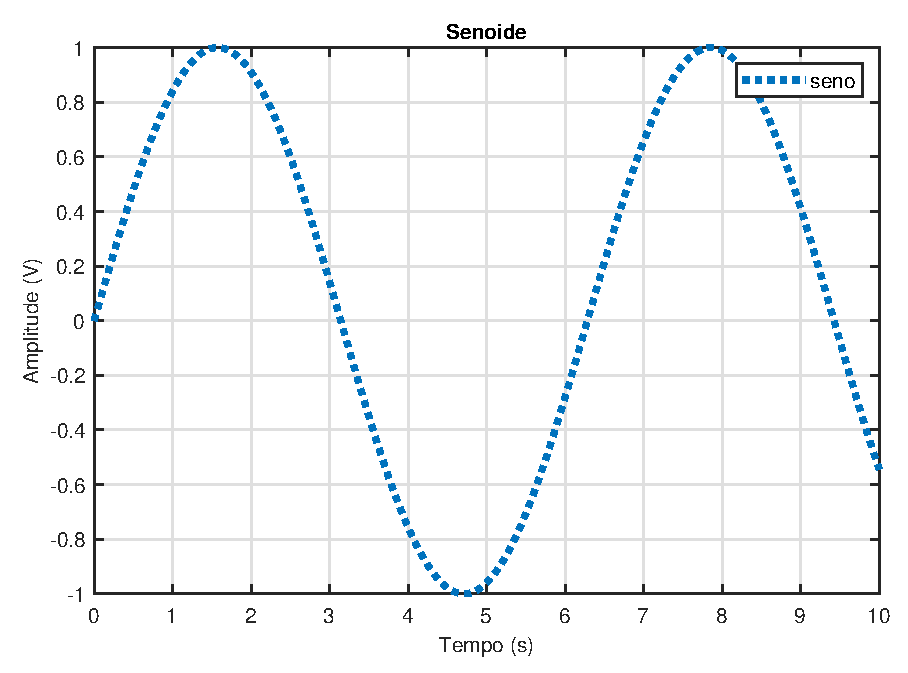
\includegraphics{teste.eps}
    \caption{Caption}
    \label{fig:enter-label}
\end{figure}

Deve Tabela~\ref{tab:jsl07} também elencar algumas equações Equação~\eqref{eq:one} de outros autores que sejam relacionados com a temática do trabalho \cite{INOUE2011}. 
Usm bom esquema para a introdução é \c{c}\~a:



\begin{itemize}
    \item Contextualização do tema (1-2 parágrafos) \cite{JESSICA2011}
    \item Motivação (1-2 parágrafos, mas pode ser junto com o objetivo e diferencial)
    \item Avaliação da literatura (3 a 5 parágrafos)
    \item Objetivo e diferencial do trabalho (1-2 parágrafos)
    \item Organização do trabalho (1 parágrafo) \cite{Joao2011}
\end{itemize}

A organização do trabalho é feita assim: “Na Seção \ref{sec:fundamentacao}, apresenta-se a fundamentação teórica do trabalho. A metodologia desenvolvida é apresentada na Seção \ref{metodologia}



\section{Metodologia}
\label{metodologia}

Nessa seção, a equipe deve relatar a metodologia empregada para a realização do trabalho, tudo aquilo que foi importante em seu desenvolvimento. Deve ser relatado também, sempre que possível, como as diferentes disciplinas abordadas no projeto integrador foram fundamentais para a solução e transposição dos problemas e das dificuldades. Mostrar o resultado final do protótipo.

\section{Fundamentação Teórica}
\label{sec:fundamentacao}

Nessa seção, são apresentados os principais conceitos teóricos utilizados no trabalho. É interessante utilizar pelo menos dois livros como referência, além de trabalhos acadêmicos. Tentar utilizar o mínimo de referências de “sites” de internet. Não inventar ou colocar nada que não tenha sido utilizado. Essa é a parte onde se confirma a relação entre as disciplinas, que foram citadas anteriormente na introdução. Caso os fundamentos teóricos sejam muito diferentes entre si, é interessante dividir a fundamentação teórica em subseções.

\begin{enumerate}
    \item primeiro
    \begin{enumerate}
        \item teste
    \end{enumerate}
    \item segundo
    \item terceiro
\end{enumerate}





\subsection{Arduino}

O arduino é uma plataforma para desenvolvimento de projetos \cite{LivroArduino}. A Figura \ref{fig:Arduino} apresenta a foto de um arduino.


\begin{figure}[H]
    \centering
    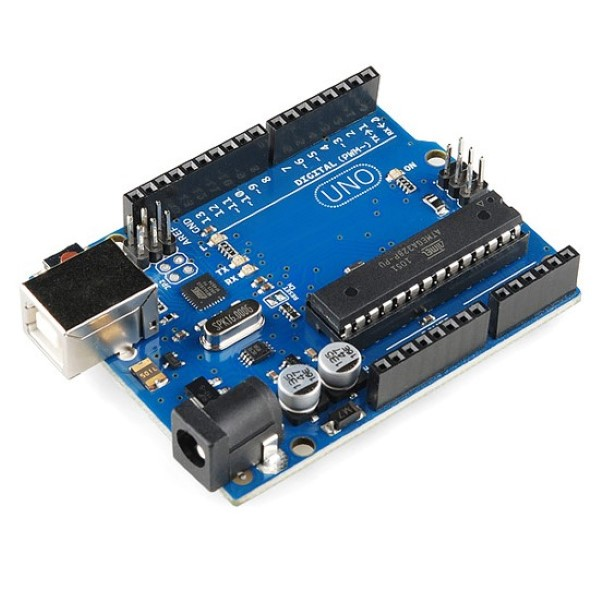
\includegraphics[width=0.5\textwidth]{Figuras/Arduino.jpg}
    \caption{blablabla}
    \label{fig:Arduino}
\end{figure}




Nessa seção, são apresentados os principais conceitos teóricos utilizados no trabalho. É interessante utilizar pelo menos dois livros como referência, além de trabalhos acadêmicos. Tentar utilizar o mínimo de referências de “sites” de internet. Não inventar ou colocar nada que não tenha sido utilizado. Essa é a parte onde se confirma a relação entre as disciplinas, que foram citadas anteriormente na introdução. Caso os fundamentos teóricos sejam muito diferentes entre si, é interessante dividir a fundamentação teórica em subseções.Nessa seção, são apresentados os principais conceitos teóricos utilizados no trabalho. É interessante utilizar pelo menos dois livros como referência, além de trabalhos acadêmicos. Tentar utilizar o mínimo de referências de “sites” de internet. Não inventar ou colocar nada que não tenha sido utilizado. Essa é a parte onde se confirma a relação entre as disciplinas, que foram citadas anteriormente na introdução. Caso os fundamentos teóricos sejam muito diferentes entre si, é interessante dividir a fundamentação teórica em subseções.Nessa seção, são apresentados os principais conceitos teóricos utilizados no trabalho. É interessante utilizar pelo menos dois livros como referência, além de trabalhos acadêmicos. Tentar utilizar o mínimo de referências de “sites” de internet. Não inventar ou colocar nada que não tenha sido utilizado. Essa é a parte onde se confirma a relação entre as disciplinas, que foram citadas anteriormente na introdução. Caso os fundamentos teóricos sejam muito diferentes entre si, é interessante dividir a fundamentação teórica em subseções.Nessa seção, são apresentados os principais conceitos teóricos utilizados no trabalho. É interessante utilizar pelo menos dois livros como referência, além de trabalhos acadêmicos. Tentar utilizar o mínimo de referências de “sites” de internet. Não inventar ou colocar nada que não tenha sido utilizado. Essa é a parte onde se confirma a relação entre as disciplinas, que foram citadas anteriormente na introdução. Caso os fundamentos teóricos sejam muito diferentes entre si, é interessante dividir a fundamentação teórica em subseções.Nessa seção, são apresentados os principais conceitos teóricos utilizados no trabalho. É interessante utilizar pelo menos dois livros como referência, além de trabalhos acadêmicos. Tentar utilizar o mínimo de referências de “sites” de internet. Não inventar ou colocar nada que não tenha sido utilizado. Essa é a parte onde se confirma a relação entre as disciplinas, que foram citadas anteriormente na introdução. Caso os fundamentos teóricos sejam muito diferentes entre si, é interessante dividir a fundamentação teórica em subseções.

\begin{figure}[!h]
  \centering
  \begin{minipage}[b]{0.4\textwidth}
    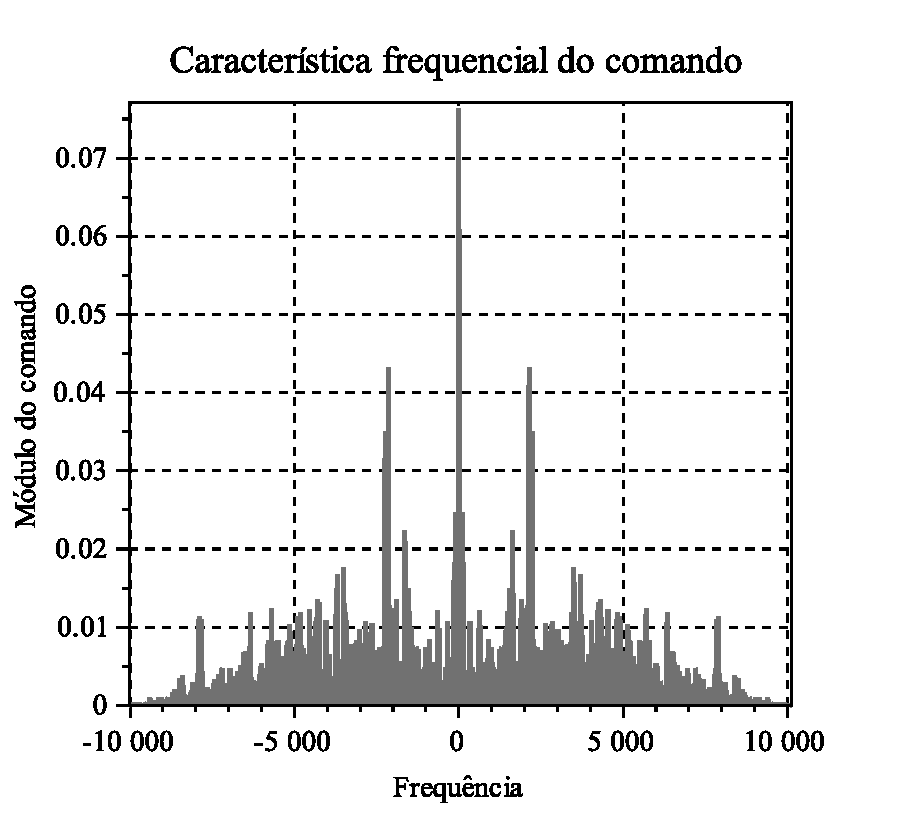
\includegraphics[width=\textwidth]{Figuras/Freq_Com.pdf}
    \caption{Flower one.}
  \end{minipage}
  \hfill
  \begin{minipage}[b]{0.4\textwidth}
    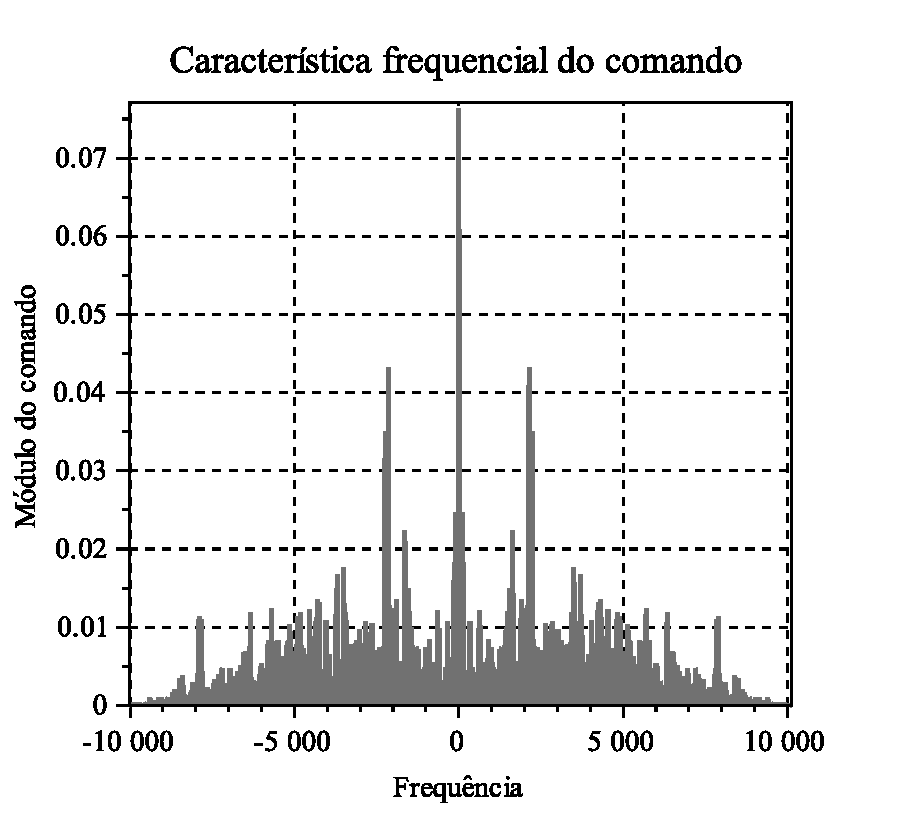
\includegraphics[width=\textwidth]{Figuras/Freq_Com.pdf}
    \caption{Flower two.}
  \end{minipage}
\end{figure}



O Teorema de Pitágoras, visto na Eq. \eqref{eq:pitagoras}, é aplicado na solução com problemas de triângulos retângulos.

O ganho de um circuito amplificador não-inversor é dado por \cite{ApostilaAldo}:

\subsection{Exemplos de equações}

As equações em LaTeX podem ser escritas assim:
\begin{equation}
    F(s) = \int_0^\infty f(t) e^{-st} \,dt. \label{eq:pitagoras}
\end{equation}


O Teorema de Pitágoras, visto na Eq. \linebreak \eqref{eq:pitagoras}, é aplicado na solução com problemas de triângulos retângulos.

O ganho de um circuito amplificador não-inversor é dado por \cite{ApostilaAldo}: %o comando \cite é utilizado para referências bibliográficas
\begin{equation}
    A = \dfrac{V_{out}}{V_{in}} = 1+\dfrac{R_f}{R}.
\end{equation}

As tensões da rede trifásica são expressas por:
\begin{align}
    v_a(t) = & \sqrt{2} V_s\cos(2\pi f t) \\
    v_b(t) = & \sqrt{2} V_s\cos\left(2\pi f t - \dfrac{2\pi}{3}\right) \\
    v_c(t) = & \sqrt{2} V_s\cos\left(2\pi f t + \dfrac{2\pi}{3}\right).
\end{align}

\subsection{Exemplos de Figuras e Tabelas}

A Figura~\ref{fig:freq} apresenta a FFT do sinal de comando de um conversor Boost.

\begin{figure}[h] %t indica topo da coluna, b indica fundo da coluna, h significa aqui nesse local, ! indica prioridade
    \centering
    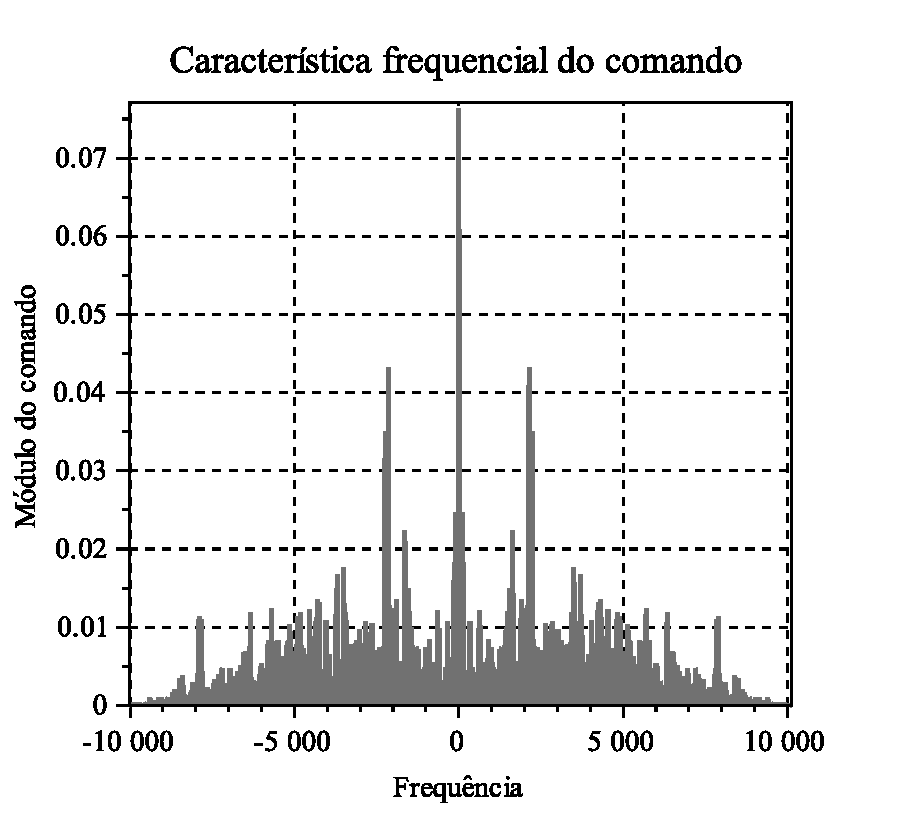
\includegraphics[width = \linewidth]{Figuras/Freq_Com.pdf}
    \caption{FFT do comando do conversor}
    \label{fig:freq}
\end{figure}




\section{Resultados}

Nesse ponto do trabalho, devem ser apresentados os resultados coletados e as discussões realizadas sobre esses dados.


\section{Conclusão}

Nas conclusões a equipe deve deixar claro se alcançou os objetivos estabelecidos no início do projeto, as principais dificuldades encontradas e aquilo que foi possível aprender com o trabalho. Deve apresentar as conclusões sobre pontos específicos e sobre o todo do trabalho.

\bibliographystyle{bib_sobraep}
\bibliography{referencias}

\end{document}
